\documentclass[../thesis.tex]{subfiles}
\begin{document}
\chapter{Introduction}\label{cap:introduction}
This chapter provides an overview of the thesis and the topics covered, from the origin of the term cloud computing to modern-day cloud computing, focusing on the serverless paradigm. Also the web crawling process will be analysed, and the ingestion phase will be studied concerning the chosen search engine.

\autoref{sec:cloud_era} defines the cloud and describes its five essential characteristics; some service models that have emerged over time are also included. In \autoref{sec:serverless}, the serverless paradigm will be analysed, considering its characteristics, advantages and issues. \autoref{sec:web_crawler} explains a general web crawler architecture and how it can be implemented according to requirements. It uses browser automation to interact with the web browser and exploits Elasticsearch \cite{site:elasticsearch} as a search engine to index the scraped HTML documents. \autoref{sec:objective_thesis} presents the objectives of this thesis and \autoref{sec:struture_thesis} explains how it is structured.

\section{The Cloud Era}\label{sec:cloud_era}
The idea of computing in a "cloud" traces back to the origins of utility computing, a concept publicly proposed in 1961 by John McCarthy, a computer scientist considered a pioneer in the field of \acrshort{AI} \cite{article:father_ai_2002}. He compared future computers with the telephone system. He said that someday the computing process might be organised as a public utility, where users share resources and have access to different services \cite{book:history_cloud_computing_2013}.

After a few decades, that the computational model had existed, it was named cloud computing. It revolutionised the world from a technological and commercial point of view, enabling companies to move away from the need for large centralised mainframes and to have on-demand computing resources made available via the Internet with consumption-based pricing. Cloud computing has become an industry game-changer, and people realise the potential of combining and sharing computing resources instead of building and maintaining them \cite{book:history_cloud_computing_2013}.

Nowadays, one of the most widely used definitions of cloud computing is given by \acrshort{NIST} \cite{article:nist_cloud_computing_2011} that provides five essential characteristics:
\begin{itemize}
    \item \textit{On-demand self-service}: a consumer can automatically access computing resources without needing human interaction with the service provider;
    \item \textit{Broad network access}: capabilities are network-accessible through standard mechanisms, facilitating use on various client platforms;
    \item \textit{Resource pooling}: provider pools computing resources, dynamically allocates them according to demand and offers location-independent access (e.g. storage, processing, memory and network bandwidth);
    \item \textit{Rapid elasticity}: capabilities can be dynamically allocated and deallocated to match demand, often seeming limitless to the consumer;
    \item \textit{Measured service}: cloud systems automatically manage and optimise the use of resources, offering transparency to service providers and consumers.
\end{itemize}

Interest in this topic has grown over the years, and the trend shown in \autoref{fig:trend_cloud_computing} demonstrates this. It is a new technology that has established itself in modern society and contributes benefits to other fields of computer science.

%\cite{article:today_tomorrow_cloud_computing_2009}
%\cite{article:perspective_study_cloud_computing_2010}

\begin{figure}[H]
    \centering
    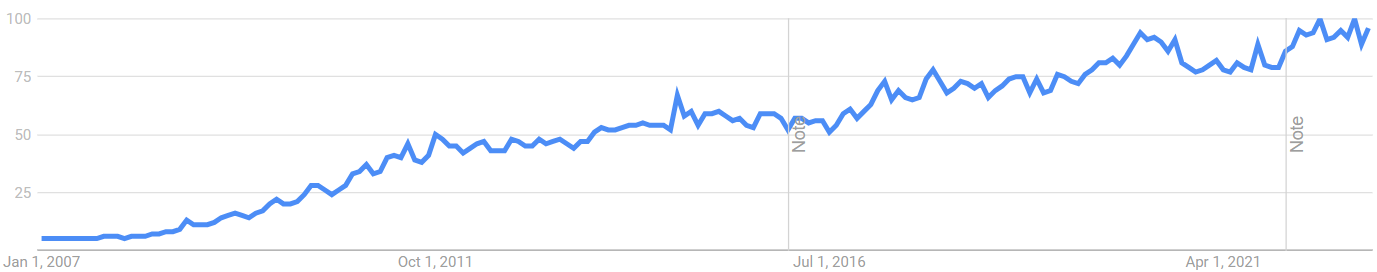
\includegraphics[width=1\textwidth]{introduction/trend_cloud_computing.png}
    \caption[Interest over time for "Cloud Computing" searches on Google]{Interest over time for "Cloud Computing" searches on Google, from 2007 to 2023. The scale is normalised from 0 to 100, with 0 representing the least popular search term and 100 representing the most popular search term. Picture from \href{https://www.google.com/trends}{Google Trends}.}
    \label{fig:trend_cloud_computing}
\end{figure}

\subsection{Cloud Service Models}
Numerous cloud services are now available, each providing varying computing resources and capabilities, as shown in \autoref{fig:cloud_service_models}. The three fundamental models are discussed by \acrshort{NIST} in \cite{article:nist_cloud_computing_2011} and then clarified in \cite{article:nist_services_evaluation_2018}. In addition, new models have been introduced in recent years, which will be analysed.

\subsubsection{Infrastructure as a Service}
The first abstraction layer gives customers instant access to cloud-based computing infrastructure such as servers, storage capacity, and networking resources. Users can configure and use them just like they would with on-premises hardware. The main difference is that the \acrfull{CSP} is responsible for hosting, managing, and maintaining the data centre's hardware and computing resources. IaaS customers can access the hardware through an internet connection and pay for their usage via a subscription or pay-as-you-go model.

Typical end users include developers and other IT professionals who require direct control over their computational resources. Some examples of IaaS are \acrlong{EC2} from \acrfull{AWS} and Compute Engine from \acrfull{GCP}.

\subsubsection{Platform as a Service}
The second abstraction layer is built over IaaS and gives customers a ready-to-use cloud platform to develop and deploy software without the complexities of managing the underlying infrastructure. Users can create, run and manage their applications using a software platform provided by another party. The provider has to take care not only of their physical resources but also of middleware, database systems, operating systems, and other supplementary services essential for the consumer application, leaving the end user in sole control of the deployed applications and their data.

Typical professional roles include developers who want to make their apps easily available. Some examples of PaaS are Elastic Beanstalk from \acrshort{AWS}, App Engine from \acrshort{GCP} and OpenShift from RedHat.

\subsubsection{Software as a Service}
The final fundamental layer at the top of the pyramid is SaaS, which provides access to applications running on a cloud infrastructure. These applications are usually accessible from various client devices using a program interface or a web browser. They can be intended as computer programs that enable the user to perform coordinated functions, tasks, or activities.

The last few decades have seen an increase in SaaS applications, such as Google Workspace (Gmail, Drive, Calendar, etc.), Slack and Netflix, which are increasingly becoming part of our daily lives.

\begin{figure}[H]
    \centering
    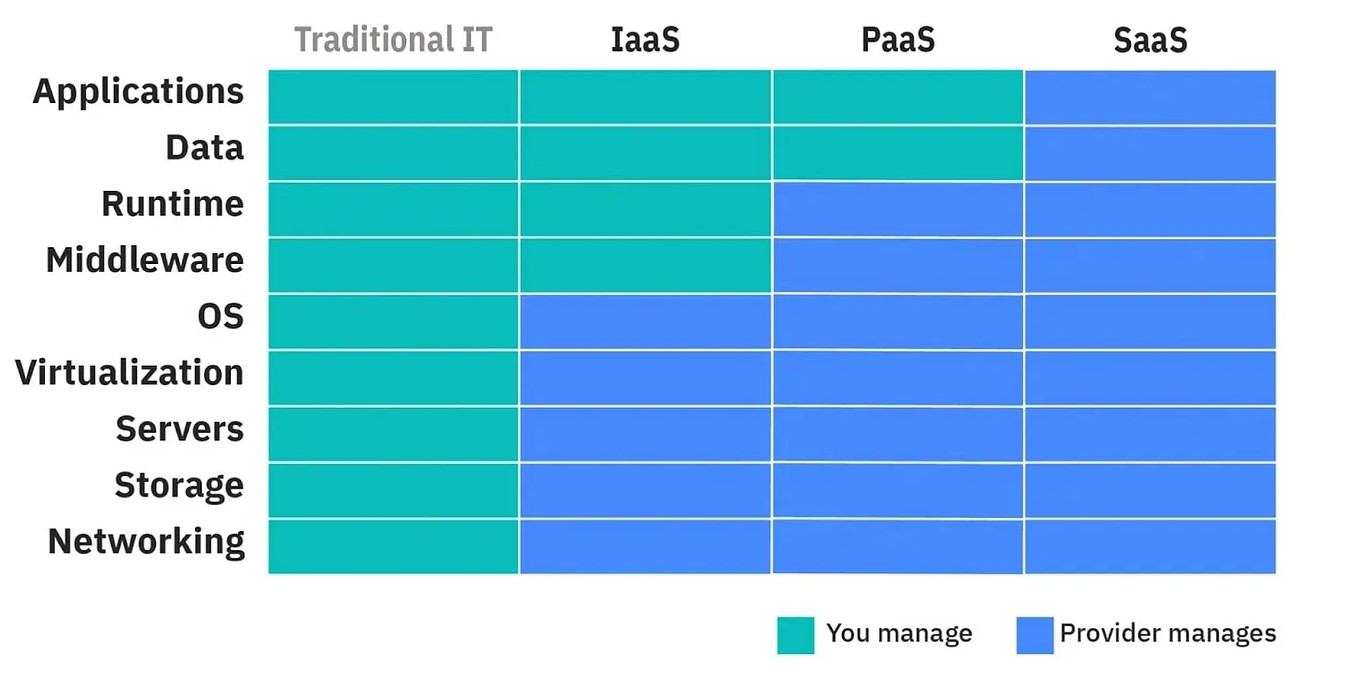
\includegraphics[width=1\textwidth]{introduction/cloud_service_models.jpg}
    \caption[Levels of abstraction of the different cloud service models]{A diagram of the different levels of abstraction in cloud service models, depicting how IaaS, PaaS, and SaaS shift management and operation obligations from the end user to the cloud provider. Picture from \href{https://blog.bytebytego.com/i/54898662/what-is-iaaspaassaas}{ByteByteGo}.}
    \label{fig:cloud_service_models}
\end{figure}

\newpage
\noindent
The following three service models aren't described by \acrshort{NIST} in \cite{article:nist_services_evaluation_2018}; they emerged in later years and helped address specific challenges and trends in software development and deployment. \acrfull{CNCF} introduces these trends in \cite{site:cncf_serverless} to better understand them and all their components.

\subsubsection{Container as a Service}
The CaaS model allows users to maintain complete control over infrastructure and get maximum portability. They can utilise container orchestration tools like \gls{k8s} \cite{article:k8s_history, site:k8s}, Docker Swarm and Apache Mesos to develop and launch portable and easily-configured applications. These tools provide flexibility and control over the app's configuration, allowing it to run on various environments without needing reconfiguration or redeployment.

Thanks to its less-opinionated application deployment model, users can enjoy maximum control, flexibility, re-usability, and ease of bringing containerised apps into the cloud. In comparison, developers have significantly more responsibility for the operating systems, load balancing, capacity management, scaling, logging and monitoring.

\subsubsection{Backend as a Service}
The BaaS model provides similar services to PaaS but also handles the typical components of an application. It simplifies the management of servers, setting up authentication, data storage, \acrshort{API}s and other backend components by abstracting their complexities. The developers must primarily focus on frontend development and application logic: the framework manages all third-party services.

Two of the most used BaaS platforms are Firebase from Google and Amplify from \acrshort{AWS}.

\subsubsection{Function as a Service}
According to \cite{inproceedings:faas_implications_2019}, the FaaS model differs from fundamentals such as IaaS and PaaS, and has significant differences to more recent models such as microservices.

It is closely related to the notion of cloud function execution, defined in \cite{article:faas_serverless_2017} as \say{a small, stateless, on-demand service with a single functional responsibility that implements specific business logic, depending on the goal of the application}. They also identify three main characteristics for them:
\begin{itemize}
    \item \textit{Short-lived}: each function takes in a typically small input and, after a typically short amount of time, produces the output;
    \item \textit{Devoid of operational logic}: the platform layer takes care of all operational matters, which allows the cloud functions to be platform-independent;
    \item \textit{Context-agnostic}: is unaware of how or why it is used.
\end{itemize}
The Function as a Service model exploits these cloud functions to enable developers with minimal experience to create, monitor and invoke them. This paradigm can be seen as serverless computing in which the cloud provider manages the resources, lifecycle, and event-driven execution of user-provided functions \cite{article:serverless_is_more_2018}.

In \autoref{sec:serverless}, the characteristics of this emerging paradigm will be explored in detail. Some examples of FaaS are Lambda from \acrshort{AWS}, Cloud Functions from \acrshort{GCP} and Knative, initially created by Google with contributions from over 50 different companies \cite{site:creator_knative}.

\section{Serverless Computing}\label{sec:serverless}
The traditional cloud computing service models have pros, but each has some cons that a software developer can perceive as complex. To ease this complexity, the cloud providers introduced a paradigm similar to PaaS, named serverless, hiding all management tasks about underlying servers for developers and allowing them more control over applications \cite{article:review_serverless_2023}.

Serverless computing describes a finer-grained deployment model that bundles applications into one or more cloud functions and uploads them to a platform which deals with the execution, scaling and billing in response to the requested demand.

With this new paradigm, consumers don't have to spend time and resources on server provisioning, maintenance, updates, scaling and capacity planning: a serverless platform takes care of all the necessary tasks and capabilities rather than being handled by individual developers or IT/operations teams. This abstraction allows developers to concentrate on writing their application's business logic while freeing up operations engineers to focus on more critical tasks for business \cite{site:cncf_serverless}.

There are two principal actors in the serverless scenario:
\begin{itemize}
    \item \textit{Developer}: writes cloud functions and benefits from the advantages of a serverless platform;
    \item \textit{Provider}: deploys the serverless platform for an internal or external client.
\end{itemize}

Although "serverless" implies that there is no need for servers, servers are still required to run a serverless platform. The platform provider manages the servers, be it virtual machines or \gls{container}s. It's worth noting that the provider will incur some cost for the running of the platform, even if there is no activity. Additionally, a self-hosted system can still be considered serverless. In this case, one team will act as the provider, while another will serve as the developer.

Usually, serverless is seen as cloud function execution, packaged as FaaS, representing the core of serverless computing. Moreover, cloud platforms also provide specialised serverless frameworks that meet specific application requirements, such as BaaS. In simple terms $serverless = FaaS + BaaS$ \cite{article:simplified_serverless_2019}.

As shown in \autoref{fig:serverless_platform}, serverless functions are designed to be triggered by specific events like \acrshort{HTTP} requests, data updates in cloud-based storage or simple notifications. These requirements concern developers who can define the rules for binding serverless functions to events. When events occur, serverless functions are triggered, and the serverless platform will automatically prepare the runtime environments. The instance initialisation, application transmission, and application code loading are all preparation processes in the runtime environments called function instances. At the end of the execution, the serverless platform automatically recycles function instances and releases corresponding resources.

\begin{figure}[H]
    \centering
    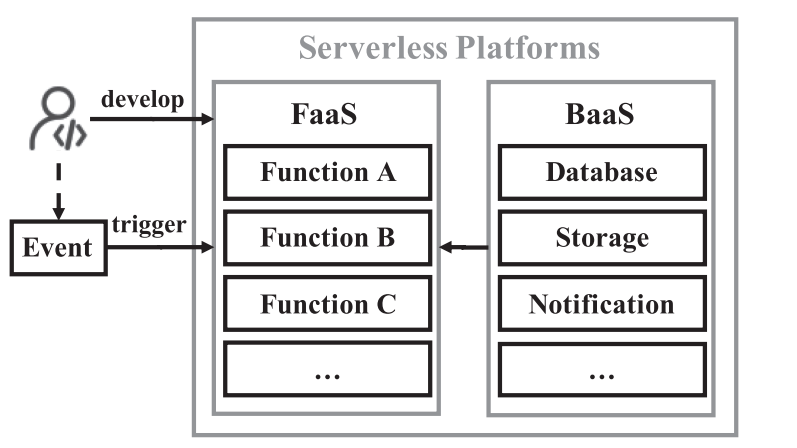
\includegraphics[width=0.75\textwidth]{introduction/serverless_platform.png}
    \caption[Development process within a serverless platform]{A diagram illustrating the development process within a serverless computing platform. Picture from \cite{article:review_serverless_2023}.}
    \label{fig:serverless_platform}
\end{figure}

To better understand serverless computing, the main features shown by the authors of \say{Rise of the Planet of Serverless Computing: A Systematic Review} \cite{article:review_serverless_2023} are described below.
\begin{itemize}
    \item \textit{Functionality and no operations}: developers can easily create applications on serverless platforms by choosing the language they are most familiar with and that suits the use case (e.g., Python, JavaScript, Java, etc.). When deploying serverless applications, developers only need to upload their application code or \gls{container} to the serverless platform, and the platform takes care of the rest;
    \item \textit{Auto-scaling}: serverless platforms can automatically adjust the number of function instances depending on the application workload dynamics. This operation is called scaling, and it allows new function instances to be started up or running occurrences to be recycled. After a request is completed, the corresponding function instances and allocated resources are stored in the memory for a short time. This prepares them to be reused by subsequent requests of the same function. Without subsequent requests, the serverless platform will scale to zero by automatically recycling these instances and resources. However, scaling down to zero creates a problem called "cold start" for new incoming requests. This is because preparing the required runtime environments from scratch takes a long time;
    \item \textit{Utilisation-based billing}: serverless computing is a pay-per-use model where software developers only pay for the resources allocated or consumed by the serverless application at the execution level. As we already said, serverless functions are event-driven and only run when triggered, allowing developers to avoid charges for idle resources. This is why the serverless paradigm is more cost-effective than traditional cloud computing, where resources need to be continuously rented;
    \item \textit{Separation of computation and storage}: the separation mode of computation and storage is adopted by serverless computing to allow the auto-scaling and the effective handling of intensive workloads;
    \item \textit{Additional limitations}: cloud providers impose additional restrictions on serverless functions to ensure the critical auto-scaling feature of serverless platforms. These limitations typically include function execution timeout, deployment package size, local disk size and maximum memory allocation. Moreover, different cloud providers have various rules concerning their serverless platforms.
\end{itemize}

In general, a serverless approach should be considered the best choice when there are processes that are easy to parallelize in independent work units and that have sporadic demand with significant, unpredictable variance in scaling requirements. Last but not least, the development time is significantly reduced to support one's evolving business.

Serverless architectures offer a new development and deployment option for cloud-native workloads that require careful consideration in the initial stages. Companies will have a high speed of change in terms of development and can handle unpredictable capacity and infrastructure requirements.  \autoref{fig:cncf_serverless} reports an overview of the serverless landscape that gives us an idea of how many realities are available and ready to use today.

\begin{figure}[H]
    \centering
    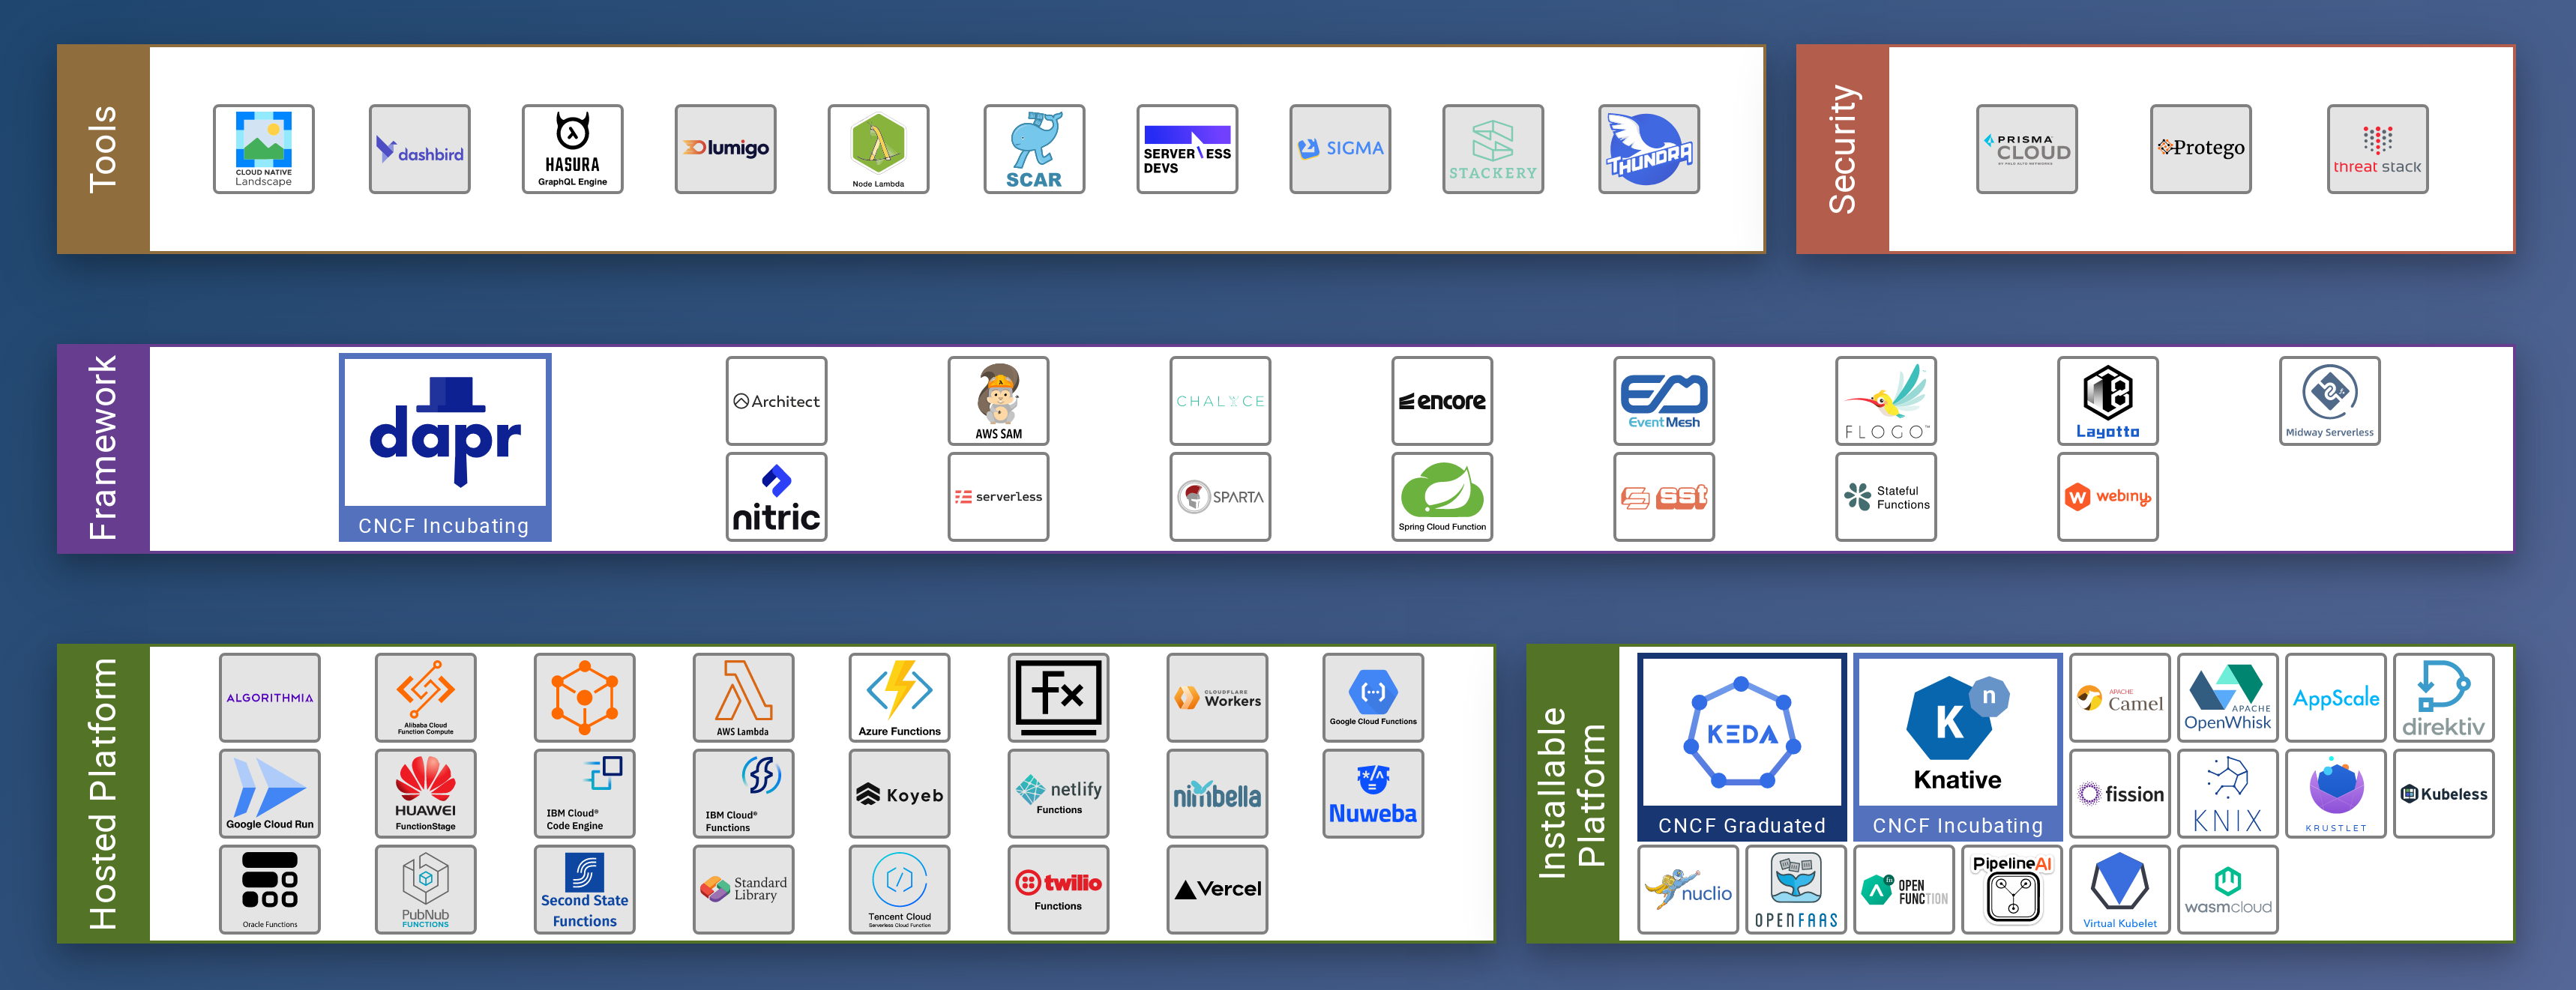
\includegraphics[width=1\textwidth]{introduction/cncf_serverless.png}
    \caption[\acrshort{CNCF} serverless landscape]{Overview of all serverless platforms, frameworks and tools categorised by \acrfull{CNCF}. Grey-coloured logos indicate non-open-source projects. Picture from \href{https://landscape.cncf.io/serverless}{CNCF}.}
    \label{fig:cncf_serverless}
\end{figure}

\subsection{Open Source Solutions}
Many \acrshort{CSP}s offer event-driven serverless platforms on their public clouds, such as \acrshort{AWS} Lambda \cite{site:aws_lambda}. These platforms allow deployment in any supported language and execute on-demand as \gls{docker} \cite{article:docker_2014} \gls{container}s.

The authors of \citetitle{inproceedings:serverless_opensource_2021} \cite{inproceedings:serverless_opensource_2021} analyse the problem of using public serverless platforms that may result in vendor lock-in risk. To avoid this risk, more and more open-source serverless platforms, which allow developers to deploy and manage functions on their self-hosted clouds, have emerged. Even so, building cloud functions requires a lot of expertise, and in order to not affect performance, an in-depth understanding of platform frameworks is necessary.

It becomes a challenge for a service developer to distinguish and select the appropriate serverless platform in different scenarios.

As shown in \autoref{fig:open_serverless_platform}, all these solutions are based on \gls{k8s} \cite{article:k8s_history, site:k8s}, a portable and extensible open-source platform that allows for the automated deployment and management of containerised workloads through declarative configuration. Many open-source serverless platforms use it to orchestrate and manage function \gls{pod}s, the atomic deployable units within \gls{k8s} \cite{article:k8s_history, site:k8s}.

\begin{figure}[H]
    \centering
    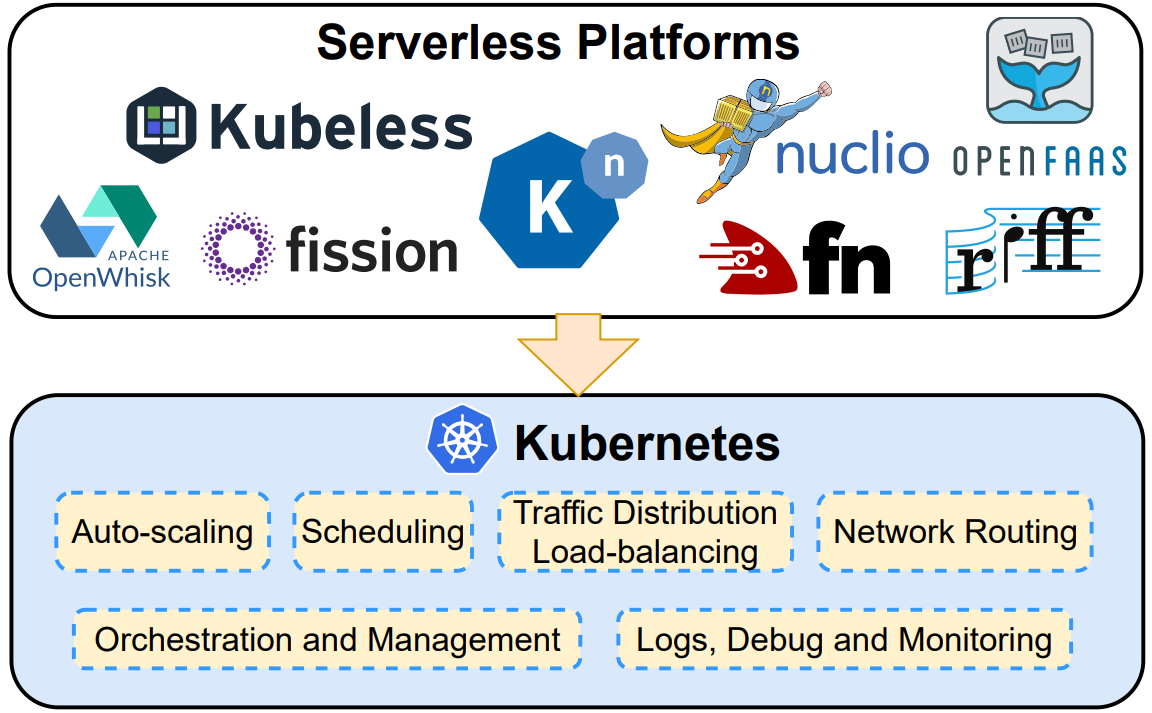
\includegraphics[width=.75\textwidth]{introduction/open_serverless_platform.png}
    \caption[Open-source serverless frameworks]{Open-source serverless frameworks and underlying \gls{k8s} services. Picture from \cite{inproceedings:serverless_opensource_2021}.}
    \label{fig:open_serverless_platform}
\end{figure}

The services in the blue box are necessary for configuration management, service discovery, auto-scaling, \gls{pod} scheduling, traffic load balancing, network routing, and service roll-out and roll-back.

\section{Web Crawler}\label{sec:web_crawler}
The \acrfull{WWW} provides abundant data in the form of \acrshort{HTML} documents. This data does not have a well-defined structure and, if site owners do not make \acrshort{API}s available, web scraping or web crawling are the fastest and most effective methods for collecting information \cite{inproceedings:cloud_web_scraping_2017, article:web_scraping_crawling_2021}.

It is necessary to distinguish between the two processes:
\begin{itemize}
    \item \textit{Web crawling}: given a seed \acrshort{URL} it downloads that web page and extracts all hyperlinks. They are needed to continue the crawling process and each visited web page is indexed to a search engine for future retrieves \cite{article:review_web_crawler_2013};
    \item \textit{Web scraping}: it enables the extraction of unstructured data from websites and transforms it into structured data, suitable for storage in a database and further analysis \cite{article:web_scraping_crawling_2021}.
\end{itemize}

Usually, they are used together to discover new web pages and extract information from them.

\subsection{Web Crawling Strategies}
According to requirements, there are different strategies for implementing a web crawler. In \cite{article:review_web_crawler_2013, article:web_crawler_types_2014}, these strategies are described and highlights are provided for each of them:
\begin{itemize}
    \item \textit{General Purpose Crawling}: a web crawler fetches pages from a set of URLs and links. It can slow down the network speed as it fetches all pages;
    \item \textit{Focused Crawling}: a focused crawler collects documents on a specific topic, reducing network traffic. It selectively looks for pages relevant to a predefined set of matters, leading to significant savings in resources;
    \item \textit{Incremental Crawling}: an incremental crawler frequently refreshes the existing collection of pages based upon the estimate as to how often pages change. It replaces less important pages with new ones that are more important, conserving network bandwidth and enriching data;
    \item \textit{Distributed Crawling}: a distributed crawler uses multiple processes to crawl and download web pages. It allows scalability based on demand;
    \item \textit{Parallel Crawling}: a parallel crawler uses multiple processes in parallel to maximize the download rate, minimize parallelization overhead, and avoid repeated downloads.
\end{itemize}

All these strategies can be performed using both libraries that send \acrshort{HTTP} requests (e.g. curl, wget, etc.) or full-featured web browser (e.g. Chrome, Firefox, etc.) that interacts directly with the \acrshort{DOM}.

\subsection{Legal Concerns}
The process of automatically extracting data from websites has become increasingly popular in both corporate and academic research projects. Web crawling and web scraping have become more accessible to perform thanks to the development of various tools and technologies. However, it is crucial to consider the legal and ethical implications of using these tools for data collection, which are rarely respected.

In \citetitle{article:web_scraping_crawling_2021} \cite{article:web_scraping_crawling_2021}, a review of the legal literature is conducted, as well as the literature on ethics and privacy, to identify areas of concern and specific issues that scholars and practitioners should address. Reflecting on these issues and concerns can help researchers reduce the risk of ethical and legal conflicts.

The legality of web crawling and scraping is still a developing area, and courts are only now beginning to handle disputes that arise from them for analytic purposes. Additionally, deciding whether web crawling or scraping for analytics raises legal issues is a highly specific determination that depends on the facts of each case. Other matters concerning the extraction of data from websites that should be addressed are described below:
\begin{itemize}
    \item It is essential to understand the language used in the service agreement or terms of use before using a website. It is important to check whether the terms allow automated access to the website, the usage of any data collected through such means, and the use of the website for purposes other than non-commercial and personal use;
    \item To use a website, users must agree to its terms. The enforceability of these terms depends on how they are presented, either through a click-wrap agreement or a prominent link to the terms-of-use page on each website;
    \item To prevent unauthorized web scraping and establish crawl rates, the robots exclusion standard protocol should be used;
    \item If the website content data is protected by copyright or not;
    \item If the website owner intends to allow or license the use of the content.
\end{itemize}

Given the rapid technological advancements in web scraping and crawling, website owners and users of these technologies must stay up-to-date regarding the law in this area.

\section{Objective of the Thesis}\label{sec:objective_thesis}
The primary purpose of this thesis is to develop a web crawler that indexes \acrshort{HTML} documents. The company Kopjra Srl \cite{site:kopjra}, where the author did his internship, was interested in collecting website information that might contain violations of reputation, intellectual or industrial property. One interesting implementation that matches both the company's and the Professor's consensus was the serverless paradigm. For this reason, testing the effectiveness of this paradigm on a web crawler application was decided upon.

Two different serverless platforms were analysed and compared: \acrshort{AWS} Lambda \cite{site:aws_lambda} and Knative \cite{site:knative}. The first is provided by \acrshort{AWS} while the latter is an open-source alternative trusted by various companies like RedHat, Google, VMWare, IBM, etc. Thanks to the horizontal scalability of this paradigm, it should be possible to reduce the execution time of each search, which is split into several concurrent cloud functions.

The third implementation follows the microservices pattern and uses the \gls{k8s} \acrshort{API} \cite{article:k8s_history, site:k8s} to create a \gls{job} that deploys a \gls{pod} for each new search. In this case, the cloud function is represented by the \gls{container} inside the \gls{pod} resource and manages the web crawling from start to end.

Following these implementations, the author exported metrics from each platform to facilitate performance comparison.

\subsection{Contributions}
The thesis outlines its main contributions in \autoref{cap:methodology}, which are summarised as follows:

\begin{itemize}
    \item Three web crawlers implementations that support both browser automation and \acrshort{HTTP} requests;
    \item The deployment of an Elasticsearch \cite{site:elasticsearch, site:elasticsearch_quickstart} cluster and the configuration of an index for the ingestion of web pages to enable keyword searches;
    \item The implementation of backend and frontend services enabling search management (i.e. creation, deletion, visualization, query);
    \item The definition of a test suite to compare the two serverless platforms and the implementation exploiting \gls{k8s} \cite{article:k8s_history, site:k8s} resources.
\end{itemize}

The latest implementation allows greater flexibility than the others, so the additional feature to perform web crawling on \acrfull{TOR} network \cite{site:tor_project} has only been developed in this one.

\section{Structure of the Thesis}\label{sec:struture_thesis}
The first chapter was necessary to introduce serverless computing and web crawling, the two central topics of this thesis.

\autoref{cap:background} illustrates the technologies required to realise the application at both the architectural and development levels.

\autoref{cap:literature_review} presents a review of web crawling applications implemented using the serverless paradigm, referring mainly to \acrshort{AWS} Lambda \cite{site:aws_lambda} and Knative \cite{site:knative} platforms.

\autoref{cap:methodology} presents the contributions of this thesis: the three proposed implementations will be analysed in detail, as well as the document ingestion, backend, and frontend services.

\autoref{cap:performance_analysis} illustrates the design of the test suite for each implementation and explains which metrics were collected. These metrics made it possible to compare results and draw performance conclusions.

The final chapter includes the conclusions of the thesis and potential future works, aiming to add new features and improve the performance side.

\end{document}